
% Pro kompilaci po částech (viz projekt.tex), nutno odkomentovat a upravit
%\documentclass[../projekt.tex]{subfiles}
%\begin{document}

\chapter{Úvod}
TODO

\chapter{Přibližné výpočetní systémy} 
\label{acs}
S rostoucím využitím výpočetních technologií v mnoha různých oblastech lidské činnosti (v posledních letech zejména rapidní rozvoj strojového učení, zpracování velkých dat, aj.), rostou také nároky na výkon a efektivitu počítačů. Zároveň se zvyšují i nároky na mobilitu výpočetních systémů, mnoho zařízení obsahuje vestavěné systémy, což omezuje možnou velikost těchto systémů.

Dle Moorova zákona se počet tranzistorů na jednom čipu každé 2 roky zhruba zdvojnásobí, ten ale pravděpodobně v dohledné době přestane vzhledem k fyzikálním vlastnostem tranzistorů platit \cite{moore}. Z tohoto důvodu je nutné se zamýšlet nad efektivnějším využitím výpočetních systémů.
Jedním z možných přístupů, který se v posledních letech těší velkému rozvoji jak ve výzkumu, tak v realné implementaci, je využití přibližných (aproximačních) výpočetních systémů.

V této kapitole bude nastíněn úvod do problematiky přibližných výpočetních systémů. Dále budou uvedeny oblasti, v nichž lze aproximaci použít a u kterých je naopak její použití nevhodné. Následují přehledy aproximačních technik, používaných hodnotících metrik a v závěru rozbor existujících přístupů k tvorbě aproximačních násobiček.

\section{Využitelnost a omezení přibližných výpočetních systémů}
Aproximační systémy lze typicky využít v oblastech, v nichž není nezbytně nutné znát přesný výsledek nějaké operace nebo výpočtu \cite{emerging_paradigm}. Takových oblastí je v informatice celá řada, zejména se jedná o zpracování multimédií, strojové učení, zpracování signálů, analýzu velkých dat, webové vyhledávače, oblast rozšířené reality, počítačové vidění, aj. Využití aproximačních technik v některých zmíněných oblastech je popsáno níže.

\subsubsection{Zpracování signálů a obrazu}
V oblasti zpracování obrazu mohou přibližné výpočetní systémy zrychlit procesy jako je např. segmentace obrazu, tedy rozdělení obrazu do částí, které korespondují s konkrétními objekty v obraze (třeba pomocí aproximace algoritmů pro detekci hran) \cite{segmentation_tech}. Dále lze aproximaci využít při zlepšování kvality obrazu, např. při zvýraznění hran nebo při odstranění šumu.

\begin{figure}[H]
    \centering
    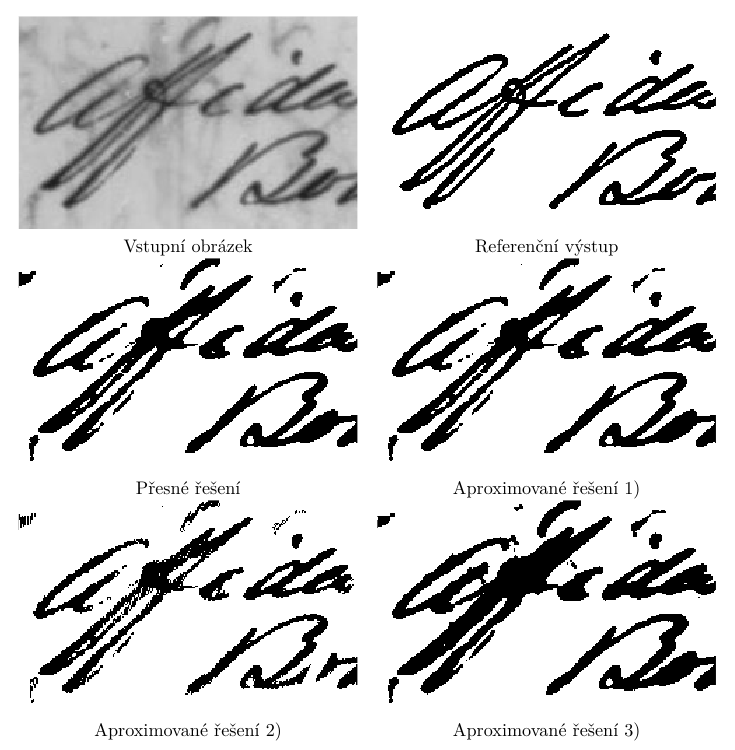
\includegraphics[width=0.9\textwidth]{obrazky-figures/approx_thresholding.png}
    \caption{Příklady výstupů aproximačních prahovacích algoritmů. Převzato z \cite{approx_image}}
    \label{fig:approx_threshold}
\end{figure}

\subsubsection{Analýza velkých dat}
Při zpracování tzv. velkých dat (angl. \textit{big data}) lze aproximovat dotazy na data, které jsou často velmi komplexní, výsledky jejich přibližných variant jsou ovšem mnohdy dostačující. Dále lze aproximovat i samotná data za účelem snížení nároků na úložný prostor. Pro nějakou třídu dotazů $Q$ na data $D$ musí platit, že pro aproximovaná data $D'$ vrátí dotazy $Q$ uspokojivé výsledky. Dotazy $Q$ bývá obvykle potřeba mírně upravit, aby vyhovovaly aproximovaným datům. V obou přístupech je třeba zvážit rovnováhu mezi efektivitou dotazů a kvalitou výsledků \cite{approx_big_data}.

\subsubsection{Strojové učení}
Přibližné počítání má ve strojovém učení (dále SU) obrovské využití, protože prostředí SU má v mnoha ohledech ideální podmínky k využítí aproximace. Mnoho úloh SU lze redukovat na problém aproximace nějaké funkce, kde daná funkce není kompletně specifikována. Samotný proces trénování modelů lze přizpůsobit tak, aby byl schopen se zotavit ze všech případných nepříznivých účinků aproximace \cite{approx_ai}.

\begin{figure}[H]
    \centering
    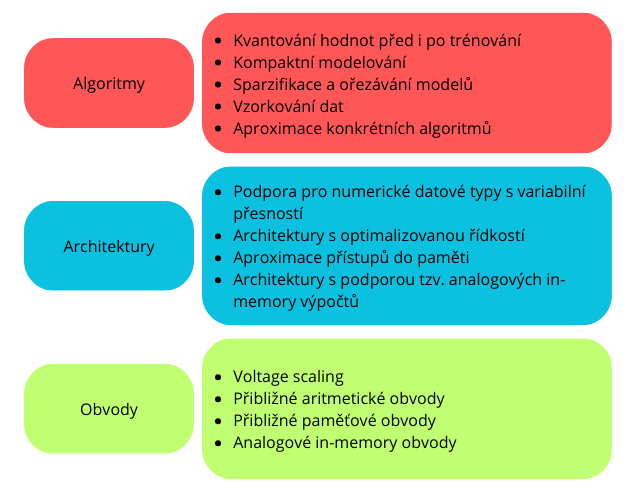
\includegraphics[width=0.7\textwidth]{obrazky-figures/ml.png}
    \caption{Přehled aproximačních technik používaných ve strojovém učení. Převzato z \cite{approx_ai}}
    \label{fig:enter-label}
\end{figure}

\subsubsection{Neaproximovatelné oblasti}
Přibližné výpočetní systémy naopak není vhodné využít tam, kde jsou z různých důvodů klíčové přesné výpočty. Typickým příkladem jsou jakékoliv peněžní transakce nebo algoritmy používané ve finančním inženýrství (angl. pojem \textit{Computational Finance}), kde by jakákoli nepřesná analýza mohla vést k velkým finančním ztrátám.

Dalším příkladem jsou tzv. bezpečnostně kritické systémy, v nichž by nepřesnosti mohly vést k ohrožení lidského života (např. systémy v automobilech, letadlech, elektrárnách apod.).

Mezi nevhodné oblasti stran aproximace lze dále řadit třeba kryptografii a šifrování, high-precision manufacturing (vysoce přesná výroba), klasické databázové systémy aj.

\section{Aproximační techniky}
V této sekci jsou stručně představeny některé používané aproximační techniky včetně uvedení jejich silných a slabých stránek a také konkrétních případů, kde je možné dané techniky využít \cite{ac_techniques}.

\subsection*{Precision scaling}
Škálování přesnosti je technika, při jejímž použití dochází ke snížení přesnosti aritmetických operací. Tuto techniku můžeme rozdělit na dva základní přístupy:
\begin{itemize}
    \item Statické škálování přesnosti -- úroveň přesnosti je stanovena na jednu předem danou hodnotu pro všechny výpočty. Tato úroveň bývá určena na základě očekávané tolerance spouštěné aplikace vůči šumu. Hlavní výhodou tohoto přístupu je jeho jednoduchost. Nevýhodou je možná nízká efektivita stran úspory energie nebo zlepšení výkonu oproti dynamickému škálování.
    \item Dynamické škálování přesnosti -- oproti statickému škálování se jedná o komplexnější techniku, při níž je úroveň přesnosti výpočtů dynamicky stanovována na základě změn tolerance spouštěné aplikace vůči šumu za běhu. Snižuje tedy přesnost výpočtů v době, kdy je tolerance vůči šumu vysoká \cite{precision_scaling}.
\end{itemize}

Obecně je tedy škálování přesnosti vhodné pro aplikace, které zpracovávají velké množství dat, která zároveň obsahují velké množství šumu.

\subsection*{Loop perforation}
Perforace smyček se zaměřuje na zrychlení provádění smyček v programu pomocí odstranění některých iterací dané smyčky. Prvním krokem při používání této techniky bývá identifikace takových smyček, jejichž zkrácením či zjednodušením nedojde k výraznému zhoršení funkčnosti programu. K tomu lze využít specializovaný kompilátor, který na základě hranice zkreslení dané uživatelem tyto smyčky identifikuje a program následně upraví \cite{code_perforation}.

Tato technika má využití v oblastech numerických výpočtů, zpracování obrazu a signálu nebo v simulacích Monte Carlo.

\begin{verbatim}
    for( i = 0; i < h; i+=4 ) { 
        /* ... */ 
    }
\end{verbatim}

\begin{verbatim}
    for( i = 0; i < h; i+=4 ) {
        if (doPerforate(i, environment)) continue;
        //...
    }
\end{verbatim}

\subsection*{Load Value Approximation}
V případě, že se procesoru nepodaří načíst data z mezipaměti (anglicky tzv. \textit{cache load miss}), je procesor nucen přistoupit k vyšším úrovním mezipaměti nebo přímo do paměti, čímž vzniká větší latence. LVA využívá aproximovatelnost některých aplikací tím, že tato data odhaduje, takže procesor může dále běžet bez větších zpoždění \cite{ac_techniques}.

Příkladem využití může být technika použitelná u grafických aplikací, kdy load-value prediktor přistupuje do paměti pouze občas (narozdíl od klasických load-value prediktorů, které přistupují do paměti při každém load miss, aby ověřily správnost své predikce). Díky tomu se výrazně sníží počet přístupů do paměti, zatímco prediktor se přesto natrénuje kvalitně \cite{load_value_approx}.

\subsection*{Memoization}
Memoizace spočívá v ukládání výstupů funkcí za účelem jejich opětovného použití při volání funkcí se stejným vstupem. Tuto metodu lze dále aproximovat znovupoužíváním těchto výstupů i u funkcí s podobným vstupem. Dochází tedy ke zrychlení díky menšímu počtu výpočtů, avšak na úkor větší paměťové náročnosti.

Memoizace je nejlépe použitelná v aplikacích, v nichž se často opakují stejné vstupy, respektive výpočty. Příkladem mohou být různé rekurzivní algoritmy, např. výpočet Fibbonaciho posloupnosti, kombinatorické vzorce nebo vyhledávací algoritmy. Přibližnou variantu memoizace lze využívat v moderních grafických aplikacích, v nichž by standardní memoizace nepřinesla významné zrychlení \cite{ac_techniques}.

\subsection*{Inexact Hardware}
Využití nepřesného hardwaru (angl. \textit{inexact hardware}) spočívá v kontrolovaném zavádění chyb do výpočetních obvodů za účelem ušetření energie, zvýšení výkonu či zmenšení plochy obvodu. Toho lze docílit např. zjednodušováním aritmetických obvodů (k tomu více v podkapitole \ref{approx_mult}).

Na obrázku \ref{fig:approx_adder} je znázorněn příklad přibližné sčítačky využívající pouze OR hradla k sečtení nejméně významných bitů \cite{log_mults}.

\begin{figure}[H]
    \centering
    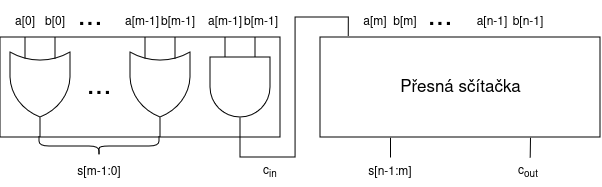
\includegraphics[width=\textwidth]{obrazky-figures/scitacka.png}
    \caption{Přibližná sčítačka lower-part-or s m nepřesnými bity. Převzato z \cite{log_mults}}
    \label{fig:approx_adder}
\end{figure}

\subsection*{Voltage Scaling}
Voltage Scaling (škálování napětí) je aproximační technika na úrovni obvodů. Jedná se o přístup, který umožňuje dynamicky měnit napětí dodávané do elektronických komponent, jako jsou mikroprocesory nebo grafické čipy, v závislosti na aktuálních požadavcích na výkon. Zvyšování napětí, tzv. \textbf{overvolting}, se používá pro zvýšení výkonu, \textbf{undervolting}, tedy snižování napětí, je využit při snaze o úsporu energie.

Při snižování napětí v obvodech mohou vznikat chyby. Například snižování napětí u paměti SRAM může vést vedle ušetření energie k častějším neúspěšným čtením a zápisům do paměti (\textit{read upset} a \textit{write failure}) \cite{ac_techniques}.

\pagebreak

\section{Hodnotící metriky} \label{error_metrics}
Jednou z klíčových otázek při implementaci aproximačních systémů je vyhodnocení míry chybovosti těchto systémů. \textbf{Chybové metriky} porovnávají výsledky přesných systémů s výsledky jejich aproximačních variant z hlediska dané metriky. Seznam některých často používaných metrik je vypsán níže \cite{circuit_library} a \cite{error_metrics}. Symbol $n_i$ v rovnicích značí počet primárních vstupů, $O_{approx}$ a $O_{orig}$ značí výstupy přibližných, respektive přesných systémů.

\bigskip

\textbf{Hammingova vzdálenost} (angl. Hamming distance, zkr. HD) mezi dvěma bitovými sekvencemi je rovna počtu pozic, na kterých se bity obou sekvencí liší \cite{hamming_dist}. Mezi používané varianty této metriky patří \textit{Průměrná Hammingova vzdálenost} nebo \textit{Maximální Hammingova vzdálenost} (v angličtině se používá výraz \textit{bit-flip error}).

Pro posuzování chybovosti násobiček není tato metoda příliš vhodná. Pokud je například očekávaný přesný výsledek výpočtu $64_{10} = 0100 0000_{2}$ a výsledek aproximace $63_{10} = 0011 1111_{2}$, jejich Hammingova vzdálenost je 7, zatímco relativní chyba je cca. $1,5 \%$.
\begin{equation}
    HD = \sum_{\forall i} OnesCount(O_{approx}^{(i)} \oplus O_{orig}^{(i)})
\end{equation}

\textbf{Pravděpodobnost chyby} (angl. error probability, zkr. EP) značí, s jakou pravděpodobností nebude výstup aproximačního systému odpovídat výstupu přesného systému.
\begin{equation}
    EP = \frac{\sum_{\forall {i:O_{approx}^{(i)} \neq O_{orig}^{(i)}}} 1} {2^{n_i}}
\end{equation}

\textbf{Průměrná absolutní chyba} (angl. mean absolute error, zkr. MAE) popisuje průměrný rozdíl mezi přesnými a přibližnými výstupy.
\begin{equation}
    MAE = \frac{\sum_{\forall i} {\left|{{O_{approx}^{(i)} - O_{orig}^{(i)}}}\right|}} {2^{n_i}}
\end{equation}

\textbf{Průměrná kvadratická chyba} (angl. mean squared error, zkr. MSE) počítá průměr druhých mocnin rozdílů mezi přesnými a přibližnými výstupy. MSE se často používá při výpočtu tzv. PSNR (zkratka z anglického \textit{Peak signal-to-noise ratio}, česky \textit{Špičkový poměr signálu k šumu}), pomocí kterého lze určovat kvalitu rekonstrukce obrázků a videí \cite{error_metrics}.
\begin{equation}
    MSE = \frac{\sum_{\forall i} {\left|{{O_{approx}^{(i)} - O_{orig}^{(i)}}}\right|^2}} {2^{n_i}}
\end{equation}

\textbf{Průměrná relativní chyba} (angl. mean relative error, zkr. MRE) uvažuje průměrnou chybu v relaci s velikostí očekávaného výstupu. Díky tomu jsou při větších hodnotách akceptovatelné větší chyby.
\begin{equation}
    MRE = \frac{\sum_{\forall i} \frac{\left|{{O_{approx}^{(i)} - O_{orig}^{(i)}}}\right|} {max(1,O_{orig}^{(i)})}} {2^{n_i}}
\end{equation}

\textbf{Nejhorší absolutní chyba} (angl. worst-case error, zkr. WCE) popisuje největší možnou chybu, které je možné při aproximaci dosáhnout.
\begin{equation}
    WCE = \max_{\forall i} \left|{O_{approx}^{(i)} - O_{orig}^{(i)}}\right|
\end{equation}

\textbf{Nejhorší relativní chyba} (angl. worst-case relative error, WCRE) uvažuje největší možnou chybu aproximačního výstupu vzhledem k očekávanému výstupu.
\begin{equation}
    WCRE = \max_{\forall i} \frac{\left|{O_{approx}^{(i)} - O_{orig}^{(i)}}\right|} {\max(1,O_{orig}^{(i)})} 
\end{equation}

\bigskip

U aproximačních obvodů jsou neméně důležité jejich \textbf{fyzické vlastnosti}. Mezi základní z nich lze zařadit zpoždění, příkon a plochu obvodu. Tyto vlastnosti je možné kombinovat v různé další složené metriky, např. PDP (z angl. \textit{Power-delay product}, tedy součin ztrát výkonu a zpoždění obvodu), ADP (z angl. \textit{Area-delay product}, tedy součin plochy a zpoždění obvodu) nebo EDP (z angl. \textit{Energy-delay product}, tedy součin zpoždění a spotřebované energie obvodu) \cite{approx_arith_circuits}.

\bigskip

Aproximační systémy je dále možné posuzovat vhodnými \textbf{kvalitativními metrikami} vzhledem k využití daného systému v konkrétní aplikaci. Mezi často používané metriky \cite{ac_techniques} patří např. výše zmíněné \textbf{PSNR}, \textbf{SSIM} (zkratka z angl. \textit{Structular similarity}, česky tedy \textit{strukturální podobnost}), \textbf{Rozdíl pixelů} (angl. \textit{Pixel difference}) nebo \textbf{UIQI} (zkratka z angl. \textit{Universal Image Quality Index}, česky tedy \textit{Univerzální index kvality obrazu}), které se používají při porovnávání podobnosti obrázků a videí.

Výstupy systémů, založených na strojovém učení nebo na shlukování, lze posuzovat např. na základě \textbf{Přesnosti} (angl. \textit{Precision}), \textbf{Výtěžnosti} (angl. \textit{Recall}), metrikou \textbf{F-score}, nebo dalších složitějších metrik \cite{clustering_eval}.

\section{Aproximační násobičky} \label{approx_mult}
Násobení je operace, která je při spouštění datově náročných aplikací (např. streamování, zpracování obrazu, strojové učení aj.) utilizována velmi často a která tím pádem spotřebuje nemalé množství energie. Mnohé z těchto aplikací jsou ovšem schopné vytvořit dostatečně dobrý výsledek i přes nepřesnosti v násobení. Dalším příkladem využití přibližných násobiček jsou zařízení z oblasti internetu věcí, u nichž je kladen důraz na co nejmenší spotřebu energie a u nichž také mnohdy není nutné vše počítat přesně \cite{approx_mult_survey}.

Tato podkapitola se zaměřuje nejprve na vysvětlení funkcionality binárních násobiček a následně na popis základních přístupů k vytváření přibližných násobiček.

\subsubsection{Základní princip binárních násobiček}
Při binárním násobení uvažujeme pouze 2 hodnoty -- 1 a 0. Z toho důvodu je možné na binární násobení nahlížet jako na sekvenci sčítání a bitových posunů. Uvažme příklad z obrázku \ref{fig:binmult}, kde vstup $x$ je násoben vstupem $y$. Operaci násobení lze rozdělit do 3 fází: načtení dat na vstupu, generování částečných součinů a finální součet.

Základní binární násobička funguje tak, že se postupně roznásobují jednotlivé bity vstupu $y$ se všemi bity vstupu $x$ a následně na základě váhy bitu $y$ dochází k bitovému posunu vlevo. První řádek částečných součinů v příkladu z obrázku \ref{fig:binmult} tedy vznikne roznásobením bitu $y_0$ se všemi bity vstupu $x$, atd. Nakonec se všechny částečné součiny sečtou v konečný výsledek.

\begin{figure}[H]
    \centering
    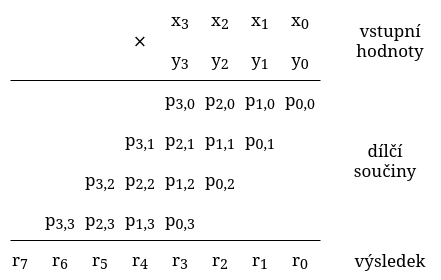
\includegraphics[width=0.55\textwidth]{obrazky-figures/binmult.png}
    \caption{Binární násobička 4x4 bity}
    \label{fig:binmult}
\end{figure}

Násobení jednotlivých bitů je implementováno jednoduše pomocí hradel AND, kritickou sekcí procesu násobení je propagace přenosu (angl. \textit{carry}) z nižšího bitu na vyšší bit. Přístupů k řešení tohoto problému je mnoho, jedním z nich je například tzv. ripple-carry sčítačka, kde se přenosy propagují postupně zprava doleva, nebo také tzv. carry-save sčítačka, kde se přenosy propagují diagonálně za účelem zrychlení výpočtu \cite{approx_mult_survey}.

\begin{figure}[H]
    \centering
    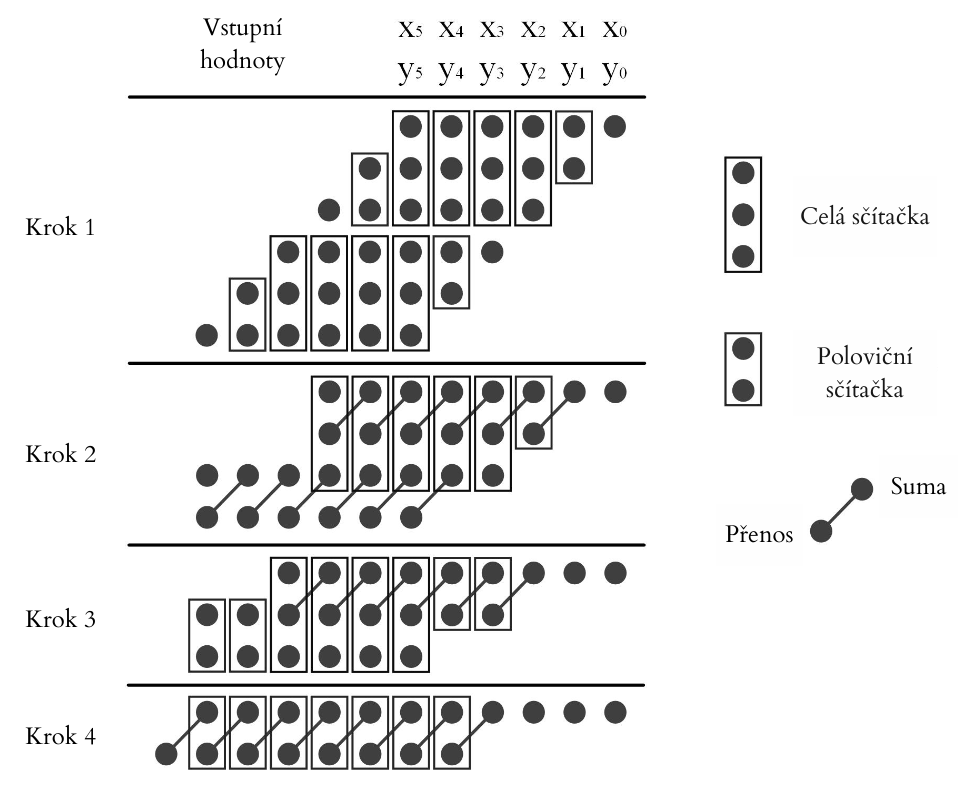
\includegraphics[width=0.75\textwidth]{obrazky-figures/wallacetree.png}
    \caption{Příklad Wallace-Tree násobičky. Převzato z \cite{approx_mult_survey}}
    \label{fig:wallacetree}
\end{figure}

Další zrychlení přináší princip tzv. Wallace Tree, v rámci něhož se seskupují 3 částečné součiny po sloupcích, které generují 2 výstupy -- sumu a přenos. Tato operace se opakuje, dokud nezůstanou poslední dva řádky částečných součinů, které se poté sečtou v konečný výsledek. V této násobičce jsou využívány úplné a částečné sčítačky, dalšího zrychlení lze docílit utilizací paralelních výpočtů \cite{wallace_tree}. Ilustrace této násobičky je na obrázku \ref{fig:wallacetree}.

\subsubsection{Aproximace vstupních hodnot}
Jednoduchým a přesto efektivním způsobem aproximace je aproximace vstupních dat. Toho lze docílit např. uříznutím několika nejméně významných bitů (zkr. LSB z angl. \textit{least significant bit}), což má menší vliv na celkový výsledek výpočtu, než uříznutí několika nejvíce významných bitů (zkr. MSB z angl. \textit{most significant bit}) \cite{approx_mult_survey}. 

Existují dvě základní metody segmentace dat -- dynamická a statická. Dynamická segmentace dat (DSM) spočívá v detekci prvního nenulového bitu a oříznutí následujících $k$ bitů. Při statické segmentaci dat (SSM) dochází k volbě jedné z předem daných strategií. Na obrázku \ref{fig:dsm_ssm} jsou ilustrovány obě metody. U SSM jsou v tomto případě následující možnosti: $k$ nejméně významných bitů, $k$ nejvíce významných bitů nebo $k$ prostředních bitů jako kompromis.

SSM zpravidla potřebuje méně hardwarových zdrojů než DSM, na druhou stranu její výsledek bývá méně efektivní, protože může obsahovat některé redundantní bity (např. nulové MSB).

\begin{figure}[H]
    \centering
    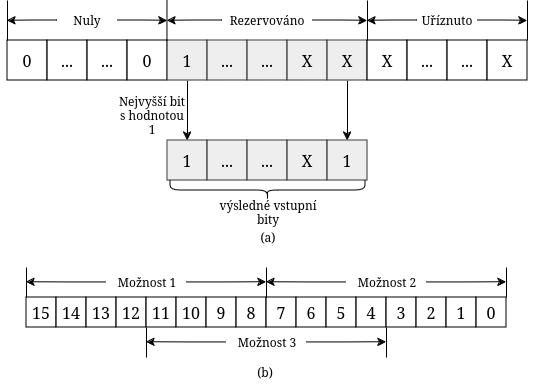
\includegraphics[width=0.8\textwidth]{obrazky-figures/dsm_ssm.png}
    \caption{(a) Příklad oříznutí DSM; (b) Příklad oříznutí SSM. Převzato z \cite{approx_mult_survey}}
    \label{fig:dsm_ssm}
\end{figure}

\subsubsection{Aproximace při generování částečných součinů}
Jedním z možných přístupů je využití malých bloků nepřesných násobiček k vytvoření dílčích součinů a poté sečtení těchto různě bitově posunutých dílčích součinů. Takové násobičky lze nazývat pojmem \textit{Nedostatečně navržená násobička} neboli anglicky \textbf{Under-designed multiplier}. 

Příkladem stavebního bloku může být násobička na obrázku \ref{fig:approx_acc_mult}. Jak lze pozorovat v Karnaughově mapě v tabulce \ref{tab:kmap2x2}, tato násobička je přesná pro 15 ze 16 možných vstupních kombinací (nepřesný výsledek je v tabulce vyznačen červeně). Změna oproti přesné násobičce je v tom, že výsledek vstupu $3\cdot3$ je reprezentován bity $111$ oproti přesnému výsledku $1001$, díky čemuž se snížila plocha obvodu téměř na polovinu (5 logických hradel oproti 9 u přesné násobičky, méně drátů) s pravděpodobností chyby pouze $\frac{1}{16}$ \cite{underdesigned_mult}.

\begin{figure}[H]
    \centering
    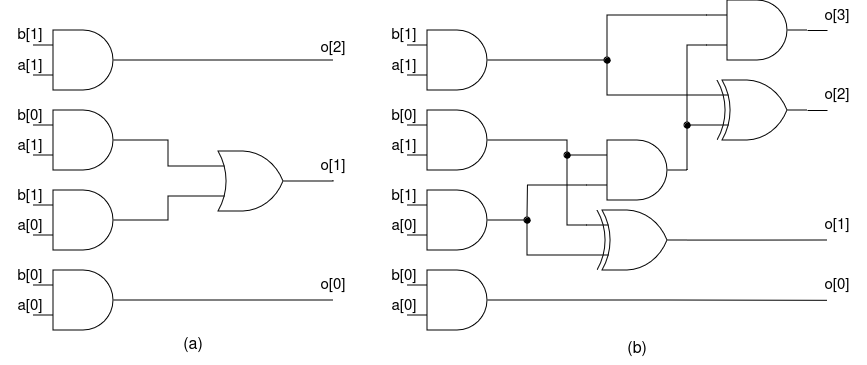
\includegraphics[width=\textwidth]{obrazky-figures/approx_acc_mult.png}
    \caption{(a) Přibližná násobička 2x2 bity (b) Přesná násobička 2x2 bity}
    \label{fig:approx_acc_mult}
\end{figure}

\begin{table}[H]
\centering
\begin{tabular}{|
>{\columncolor[HTML]{FFFFFF}}l |
>{\columncolor[HTML]{FFFFFF}}l |
>{\columncolor[HTML]{FFFFFF}}l |
>{\columncolor[HTML]{FFFFFF}}l |
>{\columncolor[HTML]{FFFFFF}}l |}
\hline
 $\times$  & 00  & 01  & 11                         & 10  \\ \hline
00 & 000 & 000 & 000                        & 000 \\ \hline
01 & 000 & 001 & 011                        & 010 \\ \hline
11 & 000 & 011 & {\color[HTML]{FE0000} 111} & 110 \\ \hline
10 & 000 & 010 & 110                        & 100 \\ \hline
\end{tabular}
\caption{Karnaughova mapa pro nepřesnou násobičku z obrázku \ref{fig:approx_acc_mult}}
\label{tab:kmap2x2}
\end{table}

Na obrázku \ref{fig:larger_mults} je znázorněn příklad násobičky 4x4 bitů složené ze 4 bloků násobiček 2x2
bity. A a X jsou vstupní hodnoty, dolní indexy H, respektive L značí 2 vyšší, respektive 2 nižší bity vstupu. V jednotlivých blocích postupně dochází k roznásobení všech kombinací dvojic vstupních bitů. Tyto dílčí výsledky jsou následně bitově posunuty a sečteny, čímž vzniká celkový výsledek násobení.

\begin{figure}[H]
    \centering
    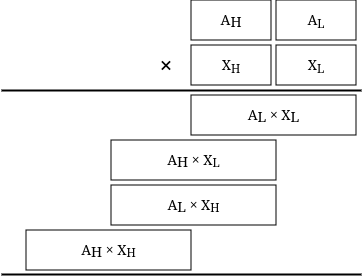
\includegraphics[width=0.5\textwidth]{obrazky-figures/larger_mults.png}
    \caption{Tvorba násobiček z menších bloků. Převzato z \cite{underdesigned_mult}}
    \label{fig:larger_mults}
\end{figure}

\subsubsection{Aproximace při závěrečném sčítání}
Pro závěrečné sčítání částečných součinů se používají sčítačky a kompresory, proto je přirozené uvažovat o aproximaci těchto komponent za účelem aproximace celé násobičky. Přístupů k tomuto řešení existuje celá řada, v posledních letech výzkumníci pracují s myšlenkou rozdělení matice částečných součinů na několik skupin (obvykle 2 nebo 3), přičemž u každé skupiny by docházelo k jinak velké aproximaci. U příkladu na obrázku \ref{fig:accumulation_approx} by nejvíce významné bity zůstaly nezměněny, prostřední bity by podléhaly určité aproximaci a nejméně významné bity by byly uříznuty nebo akumulovány pouze pomocí OR hradel.

\begin{figure}[H]
    \centering
    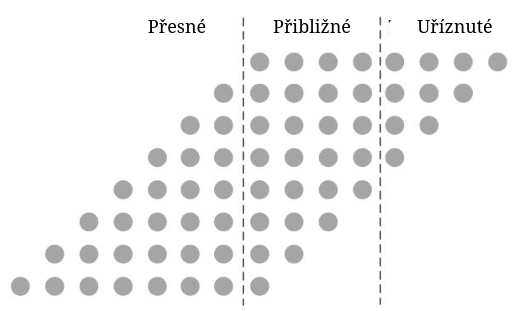
\includegraphics[width=0.6\textwidth]{obrazky-figures/accumulation_approx.png}
    \caption{Příklad rozdělení matice částečných součinů na skupiny s různou úrovní aproximace. Převzato z \cite{approx_mult_survey}}
    \label{fig:accumulation_approx}
\end{figure}

Další možností je rozdělení matice částečných součinů pomocí vertikálního a horizontálního uříznutí. Jak je vidět v příkladu na obrázku \ref{fig:bam}, všechny částečné součiny nahoru od horizontální hranice jsou při konečném součtu ignorovány. To stejné platí i pro částečné součiny napravo od vertikální hranice. Pomocí posouvání těchto hranic lze modifikovat míru aproximace. Takto navržené násobičky se nazývají anglickým pojmem \textbf{Broken-Array Multiplier}, tedy násobička s rozbitou maticí částečných součinů \cite{bio_inspired_blocks}. 

\begin{figure}[H]
    \centering
    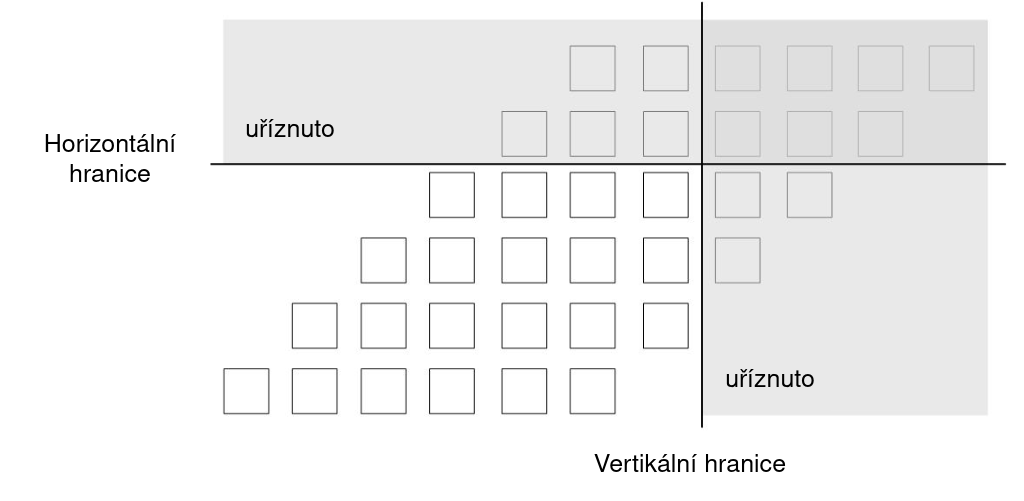
\includegraphics[width=0.85\textwidth]{obrazky-figures/bam.png}
    \caption{Příklad násobičky typu Broken-Array. Převzato z \cite{bio_inspired_blocks}}
    \label{fig:bam}
\end{figure}

\subsubsection{Logaritmické násobičky}
Násobičky lze aproximovat také na úrovni algoritmů. Jednou z možností je tvorba logaritmických násobiček, kde lze na násobení nahlížet jako na součet logaritmů obou činitelů. Při násobení čísel $A \cdot B$ lze logaritmus pro číslo $A$ vyjádřit následovně \cite{mitchell_log}:

\begin{equation}
    A = 2^{k_1}(1+x_1),
\end{equation}

\begin{equation}
    \log_2(A) = k_1 + \log_2(1+x_1),
\end{equation}

kde $A$ je činitel, $k_1$ je pozice nejvýznamnějšího bitu s hodnotou 1 a $x_1$ je desetinná část ležící v intervalu $\langle0,1)$. Stejnou formulí s parametry $k_2$ a $x_2$ lze vyjádřit i logaritmus pro činitel $B$. Logaritmus samotného násobení lze poté vyjádřit následujícím způsobem:

\begin{equation}
    \log_2(A \cdot B) = k_1 + k_2 + log_2(1+x_1) + log_2(1 + x_2)
\end{equation}

Implementace tohoto výpočtu vyžaduje použití detektoru nejvyššího jedničkového bitu (angl. \textit{Leading-one detector}), binárně-logaritmických převodníků (angl. \textit{logarithm-binary converter} a \textit{binary-logaritm converter}) a sčítačky \cite{approx_mult_survey}. Pro snížení implementační náročnosti lze výpočet aproximovat následovně:

\begin{equation}
    \log_2(x+1) \approx x, 0 \leq x < 1.
\end{equation}

Tím vzniká rovnice $A \cdot B \approx 2^{k_1+k_2+x_1+x_2} = 2^{k_1+k_2} \cdot 2^{x_1+x_2}$. Na základě přenosu z výpočtu $x_1 + x_2$ může být výpočet $A \cdot B$ dále aproximován jako:

\begin{equation}
    A \cdot B \approx \Bigg\{ 
    \begin{array}{ll}
        2^{k_1+k_2}(x_1+x_2+1) & \text{pro } x_1 + x_2 < 1, \\
        2^{k_1+k_2+1}(x_1+x_2) & \text{pro } x_1 + x_2 \geq 1.
    \end{array}
\end{equation}

Při porovnání s výsledkem přesného násobení (za předpokladu, že $x_1 + x_2 < 1$) lze chybu aproximovaného výpočtu vyjádřit jako \cite{approx_mult_survey}:

\begin{equation}
    \begin{array}{rl}
       Chyba & = A \cdot B - 2^{k_1+k_2}(x_1+x_2+1) \\
             & = 2^{k_1+k_2}(1+x_1)(1+x_2)-2^{k_1+k_2}(x_1+x_2+1) \\
             & = 2^{k_1+k_2}x_1x_2
    \end{array}
\end{equation}

\chapter{Statistické ověřování modelů}
\label{smc}
Chyby v počítačových systémech mohou mít v dnešní době drastické dopady na společnost, včetně ohrožení lidských životů, proto je dokazování správnosti těchto systémů mimořádně důležitá činnost. K verifikaci počítačových systémů tradičně existují dva základní přístupy: statická a dynamická analýza (viz obrázek \ref{fig:verifikace_rozdeleni}).

Statická analýza využívá metody formální verifikace, např. ověřování modelů, kterými lze garantovat (matematicky dokázat) bezchybnost nějakého systému. Oproti tomu dynamická analýza spočívá v simulování a testování daného systému, přičemž chyby se zachytávají při bězích jednotlivých testovacích případů. Ideální by bylo všechny systémy formálně verifikovat a zamezit tak možnosti výskytu chyby, na formální verifikaci mnohých reálných komplexních systémů ovšem nestačí výpočetní výkon současných počítačů. Tyto systémy lze ověřovat testováním, které ale pro změnu téměř nikdy neodhalí všechny chyby systému.

\begin{figure}[H]
    \centering
    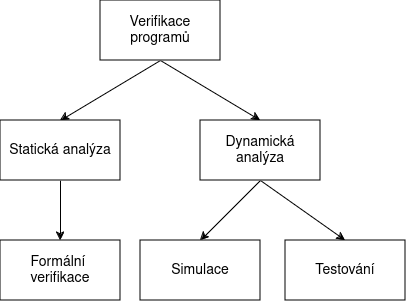
\includegraphics[width=0.5\textwidth]{obrazky-figures/verifikace_rozdeleni.png}
    \caption{Rozdělení přístupů k verifikaci programů}
    \label{fig:verifikace_rozdeleni}
\end{figure}

Metody formální verifikace se původně zaměřovaly na diskrétní chování systémů. Výzkum v posledních letech ovšem ukazuje, že spojitý (reálný) čas hraje u mnohých systémů klíčovou roli, a měl by proto být zohledněn při verifikaci. K modelování takových systémů proto vznikly časové automaty. Jedním z nejvýznamnějších nástrojů, které se prací s časovými automaty zabývají, je UPPAAL \cite{uppaal_smc}.

Časové automaty ovšem nejsou dostatečně expresivní na to, aby dokázaly popsat chování komplexnějších systémů s reálným časem. Chování těchto systémů často závisí na stochastických jevech, ověřování modelů takových systémů je nerozhodnutelné. S alternativním řešením tohoto problému přichází rozšíření UPPAAL SMC, které tyto systémy reprezentuje pomocí sítí automatů, jejichž chování může záviset na stochastických a nelineárních dynamických jevech. K efektivní analýze vlastností modelů využívá \textbf{statistického ověřování modelů}.

Tato kapitola se zabývá nejprve uvedením principu statistického ověřování modelů, poté definicí časových automatů a nakonec rozborem nástroje UPPAAL včetně jeho uživatelského rozhraní, dotazovacího jazyka a dalších rozšíření.

\section{Úvod do statistického ověřování modelů}
Tato sekce čerpá z článku \cite{uppaal_smc}. Statistické ověřování modelů (SMC) představuje určitý kompromis mezi testováním a klasickými formálními technikami ověřování modelů. Jedná se o techniku, která spočívá v monitorování simulací nějakého systému se zaměřením na určité vlastnosti a poté využití výsledků simulací k získání statistik sloužících k odhadu správnosti daného systému. Mezi používané statistické metody se řadí sekvenční testování hypotéz (\textit{sequential hypothesis testing}) nebo simulace Monte Carlo.

SMC nachází využití u systémů, které jsou příliš komplikované pro tradiční metody ověřování modelů z důvodu exploze stavového prostoru. Konkrétně se SMC využívá při ověřování systémů v biologii \cite{smc_biology}, systémů zaměřujících se na optimalizaci spotřeby energie \cite{smc_energy_centric}, v leteckém a automobilovém průmyslu i jinde. Důvodem tohoto úspěchu je relativně jednoduchá implementace a snadné pochopení a používání i pro uživatele, kteří nejsou výzkumníky v oblasti simulací a ověřování modelů. Využití statistiky také umožňuje aproximovat řešení jinak nerozhodnutelných problémů.

Mezi hlavní výhody statistického ověřování modelů lze zařadit:
\begin{itemize}
    \item Škálovatelnost -- díky tomu, že SMC neprochází celý stavový prostor, je možné ověřovat i systémy s velmi velkým až nekonečným stavovým prostorem.
    \item Efektivnost -- je výpočetně efektivnější pro systémy se složitým a stochastickým chováním, protože využívá spíše statistické odvozování oproti symbolickým výpočtům.
    \item Flexibilita -- SMC může být aplikováno na celou řadu diskrétních, spojitých i hybridních systémů.
\end{itemize}

Statistické ověřování modelů má přes své nesporné výhody i několik omezení. Přesnost výsledků závisí jak na počtu simulací, tak na správné formě dotazu a také využití správné statistické metody. Jevy, které se v chování systému objevují pouze vzácně, nemusejí být při nízkém počtu simulací objeveny a zohledněny při odvozování výsledků.

\section{Časové automaty}
Celá tato sekce čerpá z publikace \cite{mc_principles}. Časové automaty modelují chování \textbf{časově kritických systémů} (angl. \textit{time-critical system}). To jsou takové systémy, jejichž správná funkčnost nezávisí pouze na logickém výsledku nějakého výpočtu, ale také na čase, ve kterém daný výsledek vznikl. Může se jednat o ovladače zařízení v počítačích, různé komunikační protokoly a obecně systémy, které musí na něco reagovat v rámci určitého časového úseku. Díky zavedení časových omezení do automatů lze poté modelovat tvrzení jako např. \uv{Semafor se přepne na zelenou v rámci následujících 30 sekund.} Čas lze v rámci časových automatů uvažovat jak diskrétní, tak spojitý.

Časové automaty tedy zavádějí časové proměnné neboli hodiny, které se liší od běžných proměnných tím, že lze pouze sledovat jejich hodnotu nebo je resetovat na 0 (tedy nelze je nastavit na libovolnou hodnotu). Omezení, která jsou závislá na čase (tedy na hodnotách hodin), lze nazývat časovými omezeními (v angličtině \textbf{clock constraints}). Každé takové omezení odpovídá gramatice

\begin{equation*}
    g ::= x < c \hspace{0.15cm} \Big| \hspace{0.15cm} x \leq c \hspace{0.15cm} \Big| \hspace{0.15cm} x > c \hspace{0.15cm} \Big| \hspace{0.15cm} x \geq c \hspace{0.15cm} \Big| \hspace{0.15cm} g \wedge g,
\end{equation*}

kde $c \in \mathbb{N}$ a $x$ je proměnná z množiny hodin. Časová omezení, která neobsahují konjunkce, jsou atomická.

Časová omezení lze přiřazovat jak k lokacím, tak k hranám automatů, v obou případech se jejich význam liší. Časová omezení u lokací se nazývají pojmem \textbf{invariant} a značí maximální dobu, kterou může automat v dané lokaci strávit. Časovým omezením u hran se říká strážci (angl. \textbf{guard}). Ti udávají, po jaké době je možné učinit přechod po dané hraně do další lokace (tedy jak dlouho musí automat strávit v lokaci, z níž hrana vychází).

\bigskip

Časový automat je uspořádaná osmice $TA = (Loc, Act, C, \hookrightarrow, Loc_0, Inv, AP, L)$, kde

\begin{itemize}
    \item $Loc$ je konečná množina lokací,
    \item $Loc_0 \subseteq Loc$ je množina počátečních lokací,
    \item $Act$ je konečná množina akcí,
    \item $C$ je konečná množina hodin,
    \item $\hookrightarrow \hspace{0.15cm} \subseteq Loc \times CC(C) \times Act \times 2^C \times Loc$ je relace přechodu,
    \item $Inv: Loc \rightarrow CC(C)$ je funkce přiřazení invariantu (\textit{invariant-assignment function}),
    \item $AP$ je konečná množina atomických tvrzení (\textit{atomic proposition}),
    \item $L: Loc \rightarrow 2^{AP}$ je funkce označení (názvů) lokací.
\end{itemize}

Intuitivní reprezentace přechodu $\ell \xhookrightarrow{g:\alpha,D} \ell'$, kde $g$ je časové omezení, $\alpha$ je akce a $D$ je množina hodin, je následující: Automat přechází z lokace $\ell$ do lokace $\ell'$ pokud je splněno časové omezení $g$. Dále je provedena akce $\alpha$ a všechny hodiny z množiny $D$ jsou resetovány na hodnotu 0. Příklad znázornění jednoduchého časového automatu je možné vidět v následující sekci na obrázku \ref{fig:lamp}.

\section{Modelovací nástroj UPPAAL} \label{uppaal}
UPPAAL je program určený k modelování, simulaci a verifikaci systémů s realným časem. Byl vyvinut za spolupráce výzkumníků z univerzit Aalborg (Dánsko) a Uppsala (Švédsko). První vydání vzniklo v roce 1995, v době vzniku této bakalářské práce byla aktuální verze 5.0 vydaná v červnu 2023. Uživatelské rozhraní je napsáno v jazyce Java, zbytek v C++. Na C++ je také postaven jazyk používaný k deklaracím a definicím součástí modelů (k tomu více níže).

Kromě rozšíření UPPAAL SMC využívaného v této práci UPPAAL nabízí rozšíření UPPAAL Stratego zaměřující se na strategie her, UPPAAL Tiga využivající časových herních modelů (\textit{timed game automata}) k řešení her, UPPAAL CORA (zkratka z angl. \textit{Cost Optimal Reachability Analysis}) zabývající se efektivní analýzou dosažitelnosti modelů a UPPAAL TRON sloužící k tzv. black-box testování systémů s reálným časem.

\subsection{Rozšíření časových automatů v nástroji UPPAAL}
Modelovací jazyk programu UPPAAL rozšiřuje časové automaty o následující součásti \cite{uppaal_intro}:

\begin{itemize}
    \item Šablony (Templates) -- při definici automatů je možné specifikovat parametry libovolného validního datového typu, které se automatu předají jako argumenty při inicializaci.
    \item Konstanty -- Konstantní datové proměnné, pouze integer. Deklarovány jako \texttt{const name value}.
    \item Ohraničené proměnné -- proměnné deklarované jako \texttt{int[min, max] name}, kde \texttt{min} a \texttt{max} značí minimální, respektive maximální hodnotu proměnné. Tyto hranice jsou kontrolovány při verifikaci a překročení některé z nich vede k nevalidnímu stavu systému. Implicitní hranice jsou -32768 a 32768.
    \item Binární synchronizace -- využívá kanály deklarované jako \texttt{chan c}. Hrana automatu označená pomocí \texttt{c!} se synchronizuje s další hranou označenou pomocí \texttt{c?}. Hrana s otazníkem čeká na signál, hrana s vykřičníkem jej vysílá. Pokud existuje více synchronizačních kombinací, je jedna z nich vybrána nedeterministicky.
    \item Broadcastové kanály -- při broadcastové synchronizaci rozesílá jeden odesílatel \texttt{c!} signál několika příjemcům \texttt{c?} najednou. Takový kanál je deklarován jako \texttt{broadcast chan c}. Broadcastová synchronizace je neblokující, odesílatel tedy může signál vysílat i v případě, že neexistují žádní příjemci.
    \item Urgentní synchronizace -- při urgentní synchronizaci nesmí docházet k žádnému zpoždění. Hrany, které jsou označeny kanálem urgentní synchronizace, nesmí obsahovat žádná časová omezení. Kanály urgentní synchronizace jsou deklarovány jako \texttt{urgent broadcast chan c}.
    \item Urgentní a zavázané lokace -- popsány v podsekci \ref{uppaal_gui} v části \textbf{Editor}.
    \item Pole -- v UPPAALu je možné vytvářet pole hodin, kanálů, konstant a celočíselných proměnných.
    \item Funkce -- uživatelské funkce lze definovat buď globálně, nebo lokálně pro jednotlivé šablony automatů. Syntax je podobná jazyku C.
\end{itemize}

\subsection{Uživatelské rozhraní} \label{uppaal_gui}
Tato podsekce čerpá z dokumentace \cite{uppaal_doc}. Uživatelské rozhraní programu se skládá ze 4 základních součástí: editor, symbolický simulátor, konkrétní simulátor a verifikátor.

\subsubsection{Editor}
Systémový editor slouží k vytváření a úpravám modelovaného systému. Popis systému je složen z množiny šablon procesů s možnými lokálními deklaracemi, dále z globálních deklarací a nakonec systémových deklarací, v nichž dochází mimo jiné k vytvoření instancí jednotlivých šablon procesů.

Jednotlivé procesy jsou reprezentovány pomocí časových automatů, celý systém je potom tedy síť časových automatů s možností synchronizace. Modely navíc mohou obsahovat ohraničené diskrétní proměnné, se kterými lze zacházet obdobně jako s proměnnými v programovacích jazycích (čtení, zápis, aritmetické operace). Stav systému je dán aktuální pozicí (angl. pojem \textit{location}) jednotlivých automatů, aktuálním časem a hodnotami diskrétních proměnných.

Lokace jednotlivých automatů jsou značeny pomocí koleček, existují čtyři druhy:
\begin{itemize}
    \item Počáteční lokace (\textbf{initial location}) -- každý automat v UPPAALu má právě jednu, značena dvojitým kolečkem.
    \item Urgentní lokace (\textbf{urgent location}) -- pokud se automat nachází v této lokaci, zastavuje se čas. Značena písmenem U uvnitř kolečka.
    \item Zavázaná lokace (\textbf{commited location}) -- nejvíce omezující lokace, kromě zastavení času přidává podmínku, že další přechod musí být z některé ze zavázaných lokací. Značena písmenem C uvnitř kolečka.
    \item Normální lokace -- nemá žádné speciální vlastnosti.
\end{itemize}

Na obrázku \ref{fig:lamp} je ilustrován jednoduchý příklad sítě automatů reprezentující ovládání lampy. Levý automat představuje lampu, pravý automat tlačítko ovládané uživatelem. Automat lampy má 3 lokace: počáteční \texttt{off}, dále \texttt{low} a \texttt{bright}. Pro synchronizaci obou automatů je využíván synchronizační kanál nazvaný \texttt{press}. Lampa čeká (\texttt{press?} u všech hran), až uživatel stiskne tlačítko (\texttt{press!}), a následně přejde do další lokace.

Lampa obsahuje také hodiny \texttt{y}. Pokud uživatel stiskne tlačítko několikrát za sebou dostatečně rychle (\texttt{y<5}), může tím zvýšit jas lampy (přechod do lokace \texttt{bright}), při větší prodlevě se po druhém stisknutí lampa vypíná (vrací do lokace \texttt{off}) \cite{uppaal_intro}.

\begin{figure}[H]
    \centering
    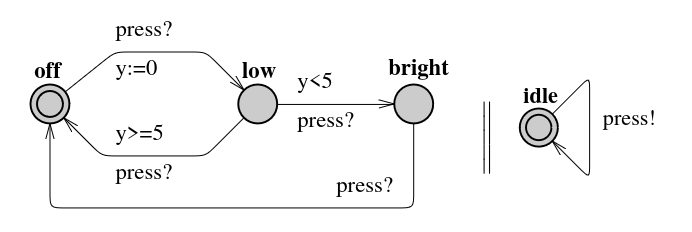
\includegraphics[width=0.8\textwidth]{obrazky-figures/lamp_model.png}
    \caption{Jednoduchý model lampy. Převzato z \cite{uppaal_intro}}
    \label{fig:lamp}
\end{figure}

\subsubsection{Symbolický simulátor a konkrétní simulátor}
\textbf{Symbolický simulátor} je nástroj určený k validaci modelovaného systému. Umožňuje spouštět běhy systému i na začátku návrhu (nebo při modelování) systému, čímž lze objevit chyby ještě před verifikací. Simulátor dále umožňuje vizualizovat běhy systému pomocí tzv. symbolických stop (angl. \textbf{symbolic traces}).

Časový automat se může nacházet v nekonečně mnoho různých stavech, tím pádem může vznikat i nekonečně mnoho konkrétních stop běhu systému. Simulátor není schopen všechny tyto stopy vizualizovat, proto zavádí symbolické stopy. Každý symbolický stav systému v symbolické stopě je sada stavů a jejich následovníků popsaná časovými omezeními. Aktivní lokace a hodnoty diskrétních proměnných jsou stejné pro všechny stavy v symbolickém stavu.

\begin{figure}[H]
    \centering
    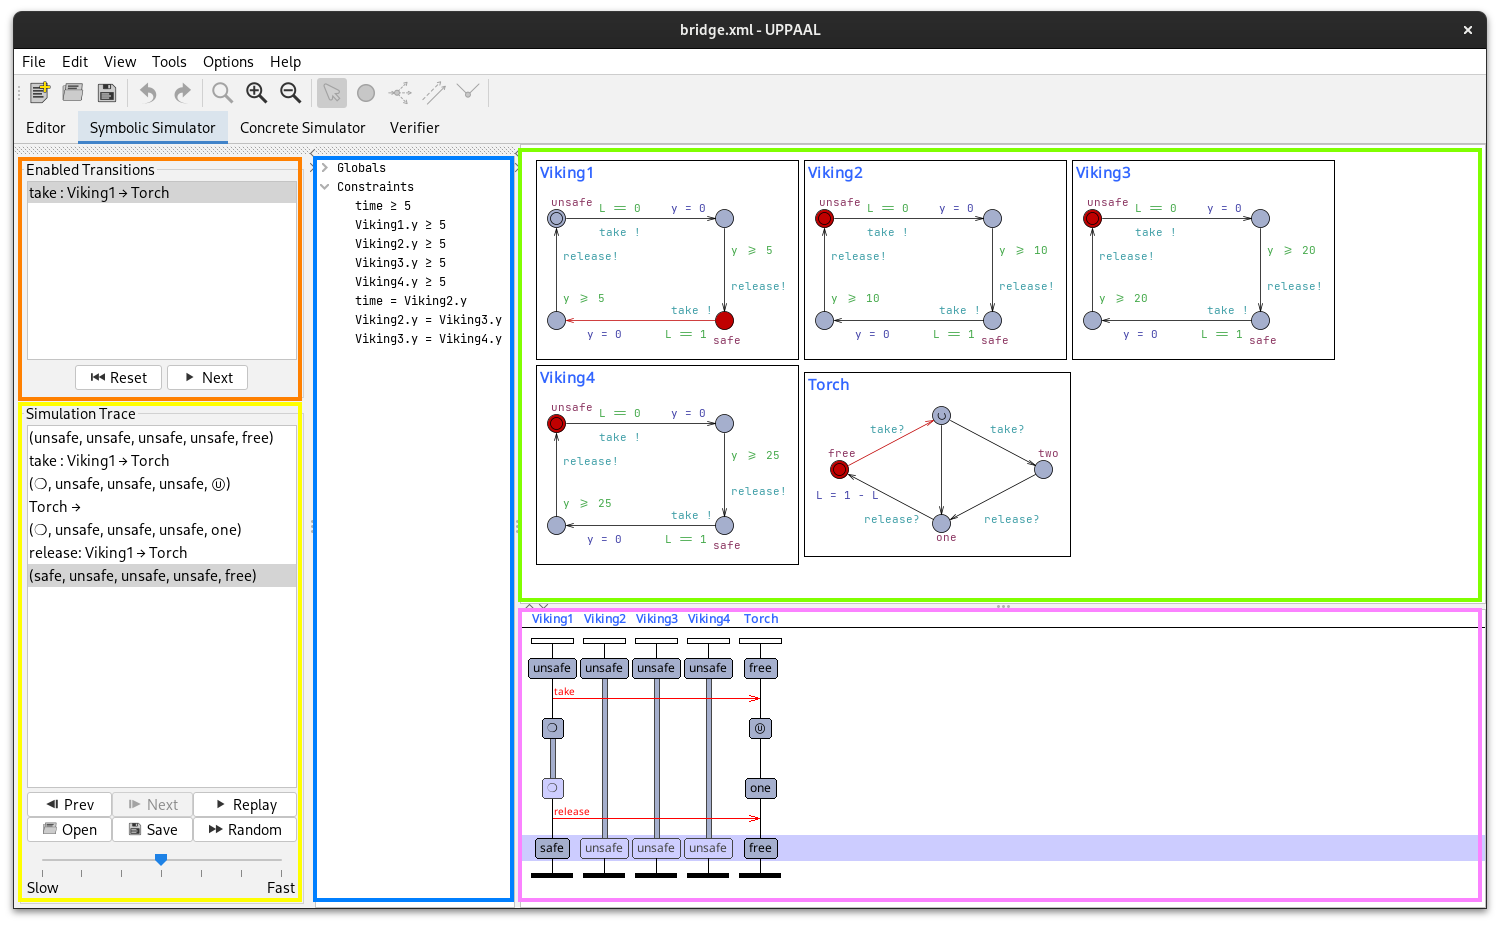
\includegraphics[width=\textwidth]{obrazky-figures/uppaal_symbsim.png}
    \caption{Symbolický simulátor v programu UPPAAL}
    \label{fig:uppaal_symbsim}
\end{figure}

Na obrázku \ref{fig:uppaal_symbsim} jsou barevně rozlišeny jednotlivé součásti simulátoru. Červená část s názvem \textit{Enabled Transitions} slouží ke krokování simulace, uživatel si sám může vybrat, který další přechod se provede. Žlutá část \textit{Simulation Trace} zobrazuje dosavadní vygenerovanou stopu. Dohromady tyto dva elementy slouží k ovládání simulace.

Prostřední modrý panel slouží k zobrazení hodnot globálních a časových proměnných ve stavu systému zvoleném ve výše popsané části \textit{Simulation Trace}. Hodnoty hodin jsou zobrazeny symbolicky jako konjunkce jednotlivých časových omezení (tedy nejsou to přesné hodnoty, ale intervaly, viz např. hodnota \texttt{time $\geq$ 5} na obrázku \ref{fig:uppaal_symbsim}).

V zelené části jsou zobrazeny jednotlivé automaty systému. Jejich aktuální lokace ve vybraném stavu jsou zvýrazněny červenou barvou. V růžové části se nachází tzv. \textit{Message sequence chart}, tedy graf sekvencí zpráv, v rámci něhož lze sledovat komunikaci a synchronizaci jednotlivých automatů systému.

\bigskip

\textbf{Konkrétní simulátor} funguje na podobném principu jako symbolický simulátor, tzn. také slouží k ranné validaci modelů. Odlišuje se tím, že simulace je založena na konkrétních stopách průchodů, takže uživatel může určit, v jaký přesný čas dochází k přechodu do dalšího stavu.

\subsubsection{Verifikátor}
Verifikátor slouží k ověřování bezpečnostních a živostních vlastností (\textit{safety and liveness properties}) systému pomocí procházení symbolického stavového prostoru reprezentovaného omezeními. Dále umožňuje specifikovat a dokumentovat požadavky na systém. Na obrázku \ref{fig:uppaal_verifier} je vidět příklad verifikátoru obsahujícího několik dotazů. Syntaxí a sémantikou dotazů se zabývají podsekce \ref{uppaal_query_lang} a \ref{uppaal_smc_queries}.

\begin{figure}[H]
    \centering
    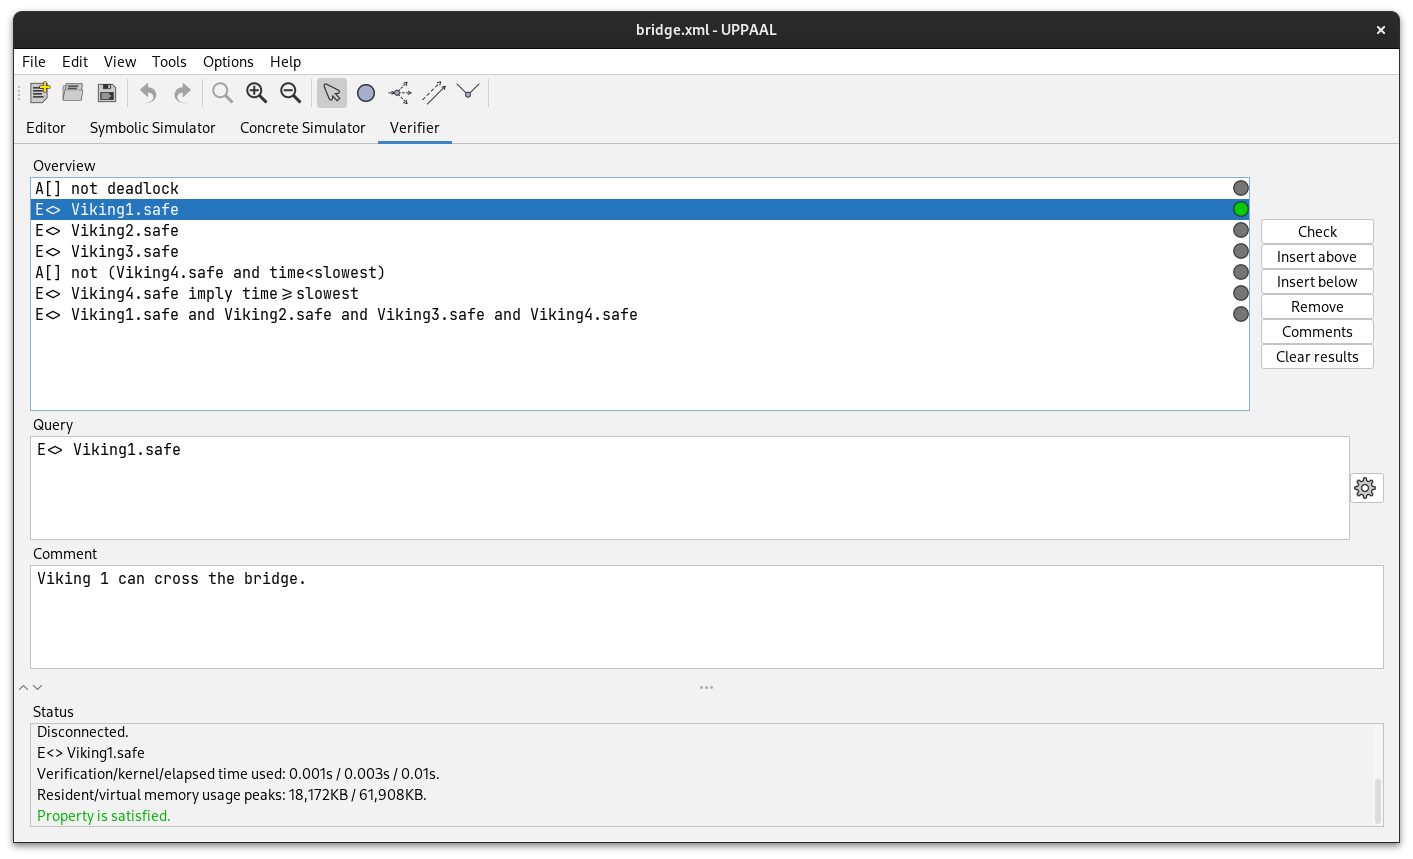
\includegraphics[width=\textwidth]{obrazky-figures/uppaal_verifier.png}
    \caption{Verifikátor programu UPPAAL}
    \label{fig:uppaal_verifier}
\end{figure}

\subsection{Dotazovací jazyk} \label{uppaal_query_lang}
Tato podsekce čerpá z článků \cite{uppaal_intro} a \cite{uppaal_smc}. Hlavním úkolem nástroje na ověřování modelů je verifikace modelu s ohledem na určité požadavky. Takové požadavky musejí být vyjádřeny v nějakém formálně definovaném a strojově čitelném jazyce. Existuje několik logik, které toto splňují, UPPAAL používá zjednodušenou verzi logiky TCTL (\textit{Timed Computation Tree Logic}). Dotazovací jazyk se tedy, podobně jako v TCTL, skládá ze stavových formulí (\textbf{state formulae}) a běhových formulí (\textbf{path formulae}). Stavové formule popisují jednotlivé stavy systému, běhové formule kvantifikují přes jednotlivé běhy nebo stopy systému.

Příklady běhových formulí lze pozorovat na obrázku \ref{fig:uppaal_path_form}. Stavy, které splňují danou stavovou formuli $\varphi$, jsou vybarveny žlutě. Hrany, které jsou procházeny při vyhodnocování, jsou ztučněny. Významy jednotlivých běhových formulí jsou vysvětleny níže ve zbytku podsekce.

\begin{figure}[H]
    \centering
    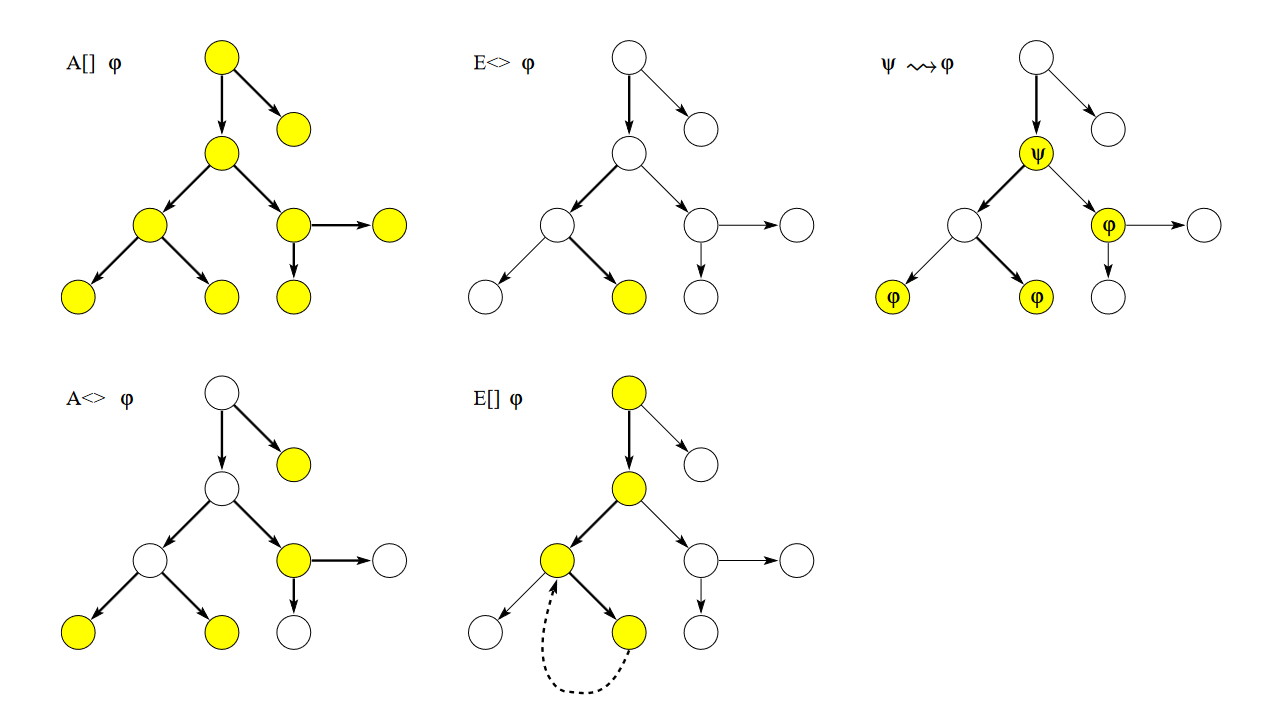
\includegraphics[width=\textwidth]{obrazky-figures/uppaal_path_form.png}
    \caption{Běhové formule v nástroji UPPAAL. Převzato z \cite{uppaal_intro}}
    \label{fig:uppaal_path_form}
\end{figure}

\subsubsection{Stavové formule}
Stavová formule je výraz, který může být vyhodnocen pro nějaký stav modelu bez ohledu na jeho chování. Příkladem může být jednoduchý výraz \texttt{i == 7}, který bude platit tehdy, pokud se v daném stavu $i$ rovná 7. Syntax stavových formulí je nadmnožinou syntaxe časových omezení, u stavových formulí je navíc možné použití disjunkce. Dále je možno otestovat, zda se proces nachází v určité lokaci pomocí výrazu \texttt{P.1}, kde \texttt{P} je proces a \texttt{1} je lokace.

\subsubsection{Dosažitelnost}
Dotazy na dosažitelnost se snaží zjistit, zda je daná stavová formule $\varphi$ splnitelná nějakým dosažitelným stavem. Jinými slovy zda existuje cesta z počátečního stavu taková, že je během ní $\varphi$ eventuelně splněno. Například při návrhu modelu nějakého komunikačního protokolu, v němž figurují odesílatel a příjemce, lze dotaz na dosažitelnost využít k ověření, že odesílatel může vůbec někdy poslat zprávu, nebo že ji příjemce eventuelně může přijmout.

K vyjádření, že by nějaký stav $\varphi$ měl být eventuelně dosažitelný, lze použít běhovou formuli $E \diamond \varphi$. V syntaxi programu UPPAAL je to \texttt{E<> $\varphi$}.

\subsubsection{Bezpečnost}
Dotazy na bezpečnost zajišťují, že nikdy nenastane \uv{něco špatného}. Příkladem může být sledování teploty v nějakém modelu elektrárny a nastavení hodnoty, přes kterou by se teplota nikdy neměla dostat. Jinou variantou tohoto dotazu je dotaz \uv{Něco se možná nikdy nestane.} Například při hraní hry je stav bezpečný, pokud v něm stále má hráč šanci vyhrát, tedy možná neprohraje.

V nástroji UPPAAL jsou tyto dotazy formulovány kladně, tedy \uv{Něco správného vždy platí.} Pro stavovou formuli $\varphi$ lze dosažitelnost ve všech stavech vyjádřit běhovou formulí $A \square \varphi$ (v syntaxi UPPAAL je to \texttt{A[] $\varphi$}). Pomocí běhové formule $E \square \varphi$ (v syntaxi UPPAAL \texttt{E[] $\varphi$}) lze vyjádřit, že by měla existovat maximální cesta taková, že $\varphi$ vždy platí. Maximální cesta je taková cesta, která je buď nekonečná, nebo končí ve stavu, z něhož nevedou žádné další přechody.

\subsubsection{Živost}
Dotazy na živost (angl. \textit{liveness}) ověřují, že se něco eventuelně stane. Například pokud došlo ke stisknutí tlačítka pro spuštění televize, že se televize eventuelně spustí, nebo že zpráva, která byla odeslána v rámci nějakého komunikačního protokolu, bude eventuelně doručena.

V nejjednodušší formě lze tyto dotazy zapisovat jako $A \diamond \varphi$, tedy že stavová formule $\varphi$ je eventuelně splněna. Složitější a užitečnější je forma dotazu $\varphi \rightsquigarrow \psi$ vyjadřující situaci \uv{Vždy, když je splněno $\varphi$, bude eventuelně později splněno i $\psi$}. V programu UPPAAL tyto dotazy zapisujeme jako \texttt{A<> $\varphi$}, respektive \texttt{$\varphi$ ----> $\psi$}.

\subsection{Rozšíření dotazovacího jazyka v rámci UPPAAL SMC} \label{uppaal_smc_queries}
Zdrojem této podsekce je článek \cite{uppaal_smc}. UPPAAL SMC rozšiřuje dotazovací jazyk o nové dotazy zaměřené na stochastickou interpretaci časových automatů. Také umožňuje uživatelům vizualizovat hodnoty výrazů a proměnných přímo v průběhu simulačních běhů. Syntax takových dotazů je následující:
\begin{equation*}
    \texttt{simulate [<=bound;N] \{ E1,...,Ek \}},
\end{equation*}
kde \texttt{N} je přirozené číslo určující počet simulací, které se mají provést, \texttt{bound} je časová hranice jednotlivých simulací a \texttt{E1,...,Ek} jsou jednotlivé výrazy, které mají být monitorovány a vizualizovány. Příkladem může být dotaz používaný v praktické části práce k vizualizaci výsledků výpočtů přesné násobičky (proměnná \texttt{res\_acc}) a zkoumané přibližné násobičky (proměnná \texttt{res\_approx}):

\begin{equation*}
    \texttt{simulate [<=20000;1] \{ res\_acc, res\_approx \}}
\end{equation*}

Výslednou vizualizaci je možno vidět na obrázku \ref{fig:simulate_example}. Nástroj UPPAAL také umožňuje export dat ve formátu csv, čehož lze využít při další podrobnější analýze.

\begin{figure}[H]
    \centering
    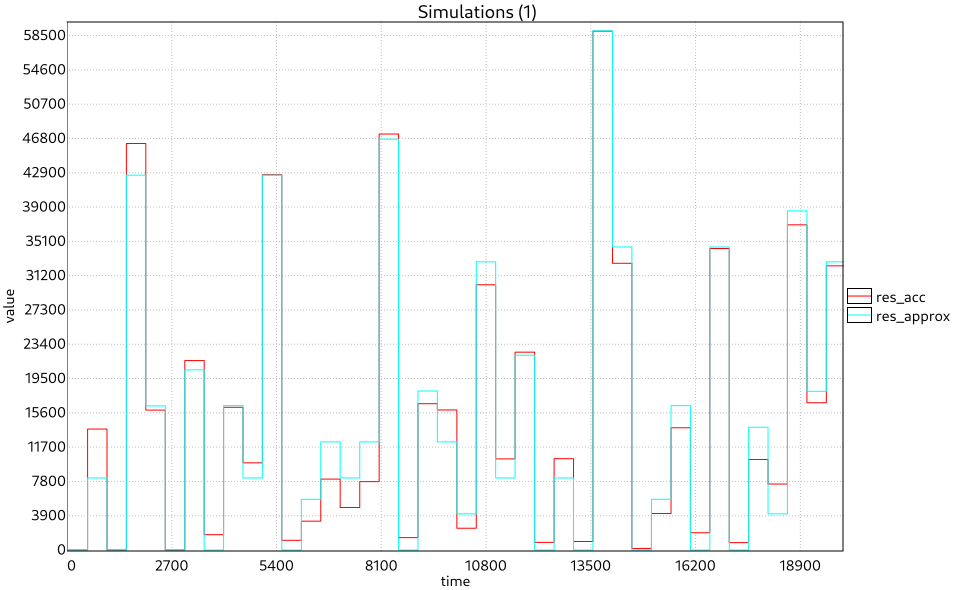
\includegraphics[width=\textwidth]{obrazky-figures/simulate_example.png}
    \caption{Vizualizace hodnot při simulaci, nástroj UPPAAL}
    \label{fig:simulate_example}
\end{figure}

\subsubsection{Odhad pravděpodobnosti}
Dotazy kvantitativního ověřování modelů mají následující syntax:

\begin{equation*}
    \texttt{Pr[<=bound;N](<>|[] expression)}
\end{equation*}

Výsledkem takového dotazu je interval spolehlivosti odhadu pravděpodobnosti, s jakou bude běhová formule \texttt{<>|[] expression} platná za předpokladu, že platí výraz \texttt{bound}. Jako hranice \texttt{bound} lze typicky zvolit nějaké časové omezení, ať už omezení globálního času, konkrétních hodin nebo třeba počet kroků (diskrétních přechodů). Konfidenční hladinu intervalu spolehlivosti lze modifikovat parametry $\alpha$ a $\epsilon$ v nastavení nástroje UPPAAL.

\subsubsection{Testování hypotéz}
Testování hypotéz, neboli kvalitativní ověřování modelů, zjišťuje, zda je pravděpodobnost platnosti nějakého výrazu vyšší nebo nižší než nějaká daná hodnota (\texttt{prob\_number}). Je efektivnější než dotaz na odhad pravděpodobnosti, protože je jednostranné, tudíž je potřeba méně simulací k dosažení stejně významného výsledku. Syntax je následující:

\begin{equation*}
    \texttt{Pr[<=bound;N] (<>|[] expression) <=|>= prob\_number}
\end{equation*}

\subsubsection{Porovnání pravděpodobností}
Tento dotaz nepřímo porovnává dvě pravděpodobnosti, aniž by je odhadoval. Syntax je následující:

\begin{equation*}
    \texttt{Pr[<=bound1;N1] (<>|[] expression1) >= Pr[<=bound2;N2] (<>|[] expression2)}
\end{equation*}

\subsubsection{Odhad hodnoty}
Umožňuje odhadnout maximální nebo minimální hodnotu určité proměnné (pouze integer nebo hodiny) v rámci časového omezení \texttt{bound}. Syntax je následující:

\begin{equation*}
    \texttt{E[<=bound;N] (min|max: expression)}
\end{equation*}

Příklad využití z praktické části práce odhaduje maximální zpoždění vzniklé při výpočtu jednoho výsledku přibližné násobičky. Časové omezení je stanoveno na 20000 jednotek, také je v dotazu explicitně stanoveno 5 simulačních běhů:

\begin{equation*}
    \texttt{E[<=20000;5] (max: current\_delay)}
\end{equation*}

Výsledkem dotazu je konfidenční interval s předem danou hladinou spolehlivosti. Výsledkem tohoto konkrétního dotazu při simulaci jedné konkrétní náhodně vybrané přibližné násobičky byla hodnota \texttt{1138 +- 18.4169 (95\% CI)}. 

Jak lze vidět na obrázku \ref{fig:prob_plots}, nástroj UPPAAL dále umožňuje některé detailnější pohledy na odhad dané hodnoty. Konkrétně se jedná o grafy rozdělení hustoty pravděpodobnosti (\textit{Probability Density Distribution}), rozdělení pravděpodobnosti (\textit{Probability Distribution}), rozdělení distribuční funkce pravděpodobnosti (\textit{Cumulative Probability Distribution}), zobrazení konfidenčních intervalů distribuční funkce (\textit{Cumulative Probability Confidence Intervals}) a také histogram frekvencí výskytu jednotlivých hodnot při simulačních bězích (\textit{Frequency Histogram}).

\begin{figure}[H]
    \centering
    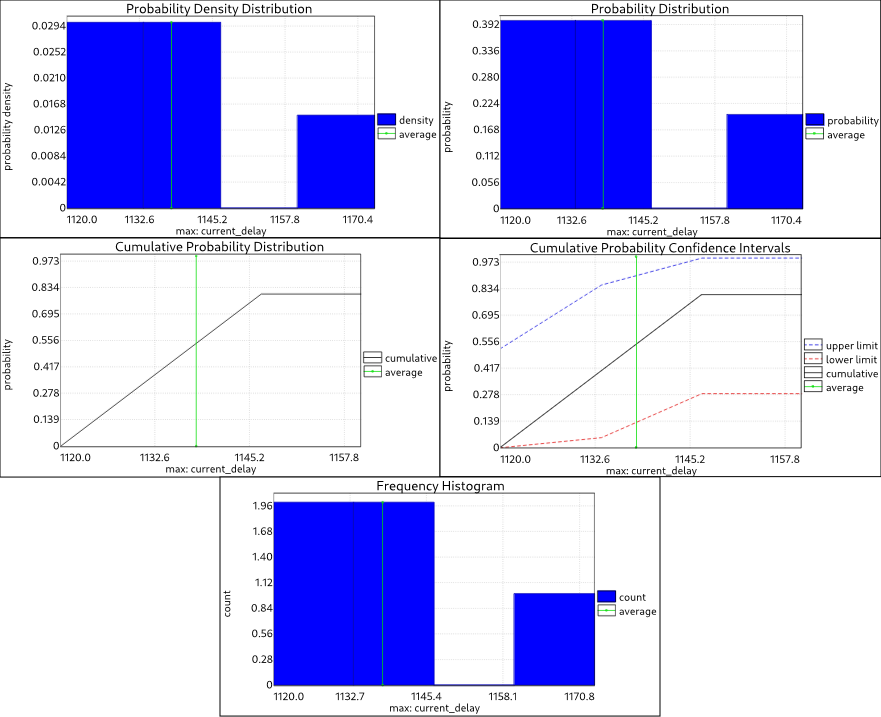
\includegraphics[width=0.9\textwidth]{obrazky-figures/prob_plots.png}
    \caption{Grafy pravděpodobnostního rozdělení při odhadu maximální hodnoty proměnné v nástroji UPPAAL}
    \label{fig:prob_plots}
\end{figure}

\chapter{Návrh a implementace řešení}
\label{rozbor}
Hlavním cílem praktické části bakalářské práce bylo vytvoření modelů zástupců zvolené třídy přibližných výpočetních systémů (angl. \textit{Approximate Computing}, zkratka AC), ověření jejich vlastností pomocí prostředků SMC a porovnání těchto vlastností s vlastnostmi přesných variant daných výpočetních systémů.

Jako třída zkoumaných AC systémů byly zvoleny násobičky. Práce navazuje zejména na článek \cite{smc_axc}, tedy na práci vedoucího této bakalářské práce dr. Strnadela. Konkrétně přebírá systém modelů sloužící k simulaci násobení přesné a přibližné násobičky 2x2 bity a rozšiřuje jej o následující prvky:
\begin{itemize}
    \item rozšíření systému pro větší násobičky (až 11x11 bitů),
    \item výpočet chybových metrik popsaných v části \ref{error_metrics},
    \item sledování počtu překlopení bitů (\textit{bit flips}) při jednotlivých výpočtech,
    \item sledování zpoždění při jednotlivých výpočtech,
    \item generování vstupů s různým pravděpodobnostním rozdělením.
\end{itemize}

Jako zdroj modelů přibližných násobiček byla zvolena knihovna EvoApproxLib \cite{circuit_library}. Tato knihovna poskytuje dohromady několik stovek modelů přibližných násobiček a sčítaček jak v bezznaménkové, tak znaménkové variantě. Tato práce se zaměřuje na bezznaménkové násobičky, zejména na variantu 8x8 bitů, ale implementovaný překladač (viz sekce \ref{parser}) lze použít i pro násobičky 7x7 a 11x11 bitů.

\bigskip

Předmětem zkoumání bylo porovnávání vlastností přibližných násobiček při generování vstupních hodnot podle různých pravděpodobnostních rozdělení. Základní osnova postupu řešení vypadala následovně:

\begin{itemize}
    \item nasbírání dat (násobených dvojic čísel) z vybraných algoritmů, vizualizace dat,
    \item tvorba pravděpodobnostních rozdělení pro generování náhodných čísel podle reálných rozdělení násobených čísel v implementacích algoritmů,
    \item implementace \uv{překladače}, který převádí modely přibližných násobiček z knihovny \cite{circuit_library} napsaných v jazyce Verilog do modelů v nástroji UPPAAL,
    \item vytvoření simulačních dotazů ve verifikátoru nástroje UPPAAL,
    \item simulace různých kombinací násobiček a náhodných rozdělení, 
    \item zpracování a vizualizace výsledků.
\end{itemize}

Tato kapitola se zabývá podrobnějším popisem návrhu a řešení výše zmíněných bodů.

\section{Popis systému v nástroji UPPAAL}
Tato sekce se věnuje popisu systému modelů v nástroji UPPAAL. Zaměřuje se především na popis jednotlivých modelů -- časových automatů, dále jsou zmíněny některé důležité proměnné a funkce a také je nastíněna celková synchronizace systému.

\subsection{Globální deklarace}
V rámci globálních deklarací dochází k vytvoření základního rozhraní systému. Nejdůležitější součásti jsou zobrazeny ve výpise \ref{lst:interface}. 

Jedná se o definici počtu vstupních a výstupních bitů systému (tedy kolik bitů mají 2 vstupní hodnoty a kolik bitů má 1 výstupní hodnota) v proměnných \texttt{NPI}, resp. \texttt{NPO}. Dále je deklarováno pole pravdivostních hodnot \texttt{bits}, které slouží jak uložení bitů vstupních a výstupních hodnot, tak také k uložení dílčích výstupů jednotlivých logických hradel. Každé hradlo má svoje unikátní ID, které slouží jako index do pole \texttt{bits}, kam ukládá výsledek svojí operace, a odkud jej poté mohou další hradla načíst.

Indexy bitů vstupních a výstupních hodnot jsou definovány v polích \texttt{PIxy}, respektive \texttt{POx} (výstup přesné násobičky) a \texttt{POy} (výstup přibližné násobičky).

\begin{lstlisting}[language={C}, caption={Základní rozhraní systému}, label={lst:interface}]
const NPI = 16; //number of input bits
const NPO = 16; //number of output bits

const int MAX_BITS = 1024;
bool bits[MAX_BITS];

//indexes of input bits for both input numbers
const int PIxy[NPI] = {0, 1, 2, 3, 4, 5, 6, 7, 8,
    9, 10, 11, 12, 13, 14, 15};

//indexes of bits of accurate mult. output
const int POx[NPO] = {16, 17, 18, 19, 20, 21, 22,
    23, 24, 25, 26, 27, 28, 29, 30, 31};

//indexes of bits of approx. mult. output
const int POy[NPO] = {32, 33, 34, 35, 36, 37, 38,
    39, 40, 41, 42, 43, 44, 45, 46, 47};
\end{lstlisting}

Dále zde dochází k deklaracím a definicím řady pomocných proměnných a funkcí, zejména všech proměnných obsahujících výsledky výpočtů sledovaných chybových metrik, také funkce porovnávající výsledky výpočtů přesné a přibližné násobičky aj.

\subsection{Modely}
V této podsekci jsou zobrazeny a popsány jednotlivé používané modely.

\subsubsection{Model přesné násobičky}
Modeluje kombinační obvod přesné násobičky definovaný pomocí pravdivostní tabulky. Po inicializaci model čeká na signál kanálu \texttt{update}, který značí vygenerování nových vstupních hodnot. Poté v rámci funkce \texttt{f()} vygeneruje výsledek výpočtu pro kombinaci vstupů a pravdivostní tabulky a uloží jej do globální proměnné \texttt{bits}. Po uběhnutí \texttt{dly} časových jednotek se vrací do stavu čekání na další vstupní hodnoty.

\begin{figure}[H]
    \centering
    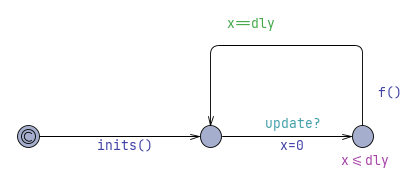
\includegraphics[width=0.6\textwidth]{obrazky-figures/model_tmul2any.png}
    \caption{Časový automat reprezentující model přesné násobičky}
    \label{fig:model_tmul2any}
\end{figure}

\subsubsection{Model generátoru vstupů}
Model generátoru pseudonáhodných čísel -- dvou vstupních hodnot pro přesnou i přibližnou násobičku. Po inicializaci model pomocí funkce \texttt{f(idx)} vygeneruje nové hodnoty a rozešle synchronizační signál v kanále \texttt{update}. Pomocí funkce \texttt{inCovered} sleduje, zda byly vygenerovány všechny možné vstupní kombinace. Pokud ano, ukončuje generování a přechází do lokace \texttt{done}. Jinak čeká na signál z kanálu \texttt{cmpDone} a poté generuje další dvojici hodnot.

\begin{figure}[H]
    \centering
    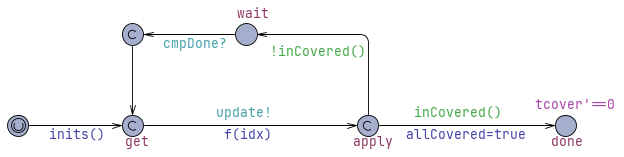
\includegraphics[width=0.9\textwidth]{obrazky-figures/model_tmul2_tb_random.png}
    \caption{Časový automat reprezentující model generátoru pseudonáhodných veličin}
    \label{fig:model_tmul2_tb_random}
\end{figure}

\subsubsection{Model kontroly rovnosti}
Tento model provádí kontrolu rovnosti výsledků přibližné a přesné násobičky. Model čeká ve své počáteční lokaci, dokud nejsou připraveny výsledky jak přesného, tak přibližného výpočtu (\texttt{diffctrl==2}). Poté v rámci volání funkce \texttt{diff()} provede porovnání výsledků a také průběžné výpočty všech sledovaných metrik. Po dokončení všech výpočtů odesílá signál v kanále \texttt{cmpDone} značící, že porovnávání bylo dokončeno, a vrací se do počáteční lokace.

\begin{figure}[H]
    \centering
    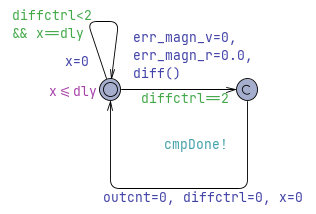
\includegraphics[width=0.45\textwidth]{obrazky-figures/model_eval_diff.png}
    \caption{Časový automat reprezentující model kontroloru rovnosti výsledků}
    \label{fig:model_eval_diff}
\end{figure}

\subsubsection{Model synchronizace vstupních hodnot}
Model čeká na vygenerování nových vstupních hodnot (tedy na signál \texttt{update?}). Poté pomocí kanálu \texttt{change[idx]} postupně dává signál jednotlivým logickým členům, že byl jejich vstupní bit aktualizován. Proměnná \texttt{idx} představuje pozici jednotlivých bitů. Model iteruje mezi dvěma zavázanými lokacemi tak dlouho, dokud se neprojde přes všechny vstupní bity (konstantní proměnná \texttt{NPI} značí počet vstupních bitů násobičky). Po aktualizování všech bitů se model vrací do počáteční lokace.

\begin{figure}[H]
    \centering
    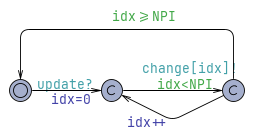
\includegraphics[width=0.4\textwidth]{obrazky-figures/model_syncPrimary.png}
    \caption{Časový automat reprezentující model zajišťující synchronizaci vstupních hodnot}
    \label{fig:model_syncPrimary}
\end{figure}

\subsubsection{Model logického hradla}
Modeluje logický člen se dvěma vstupy a jedním výstupem. Model při inicializaci přijímá následující vstupní parametry:
\begin{equation*}
    \begin{array}{l}
       \texttt{const int id, const int a0, const int a1, const int y0,} \\
       \texttt{broadcast chan \&cin0, broadcast chan \&cin1, broadcast chan \&cout0,}
    \end{array}
\end{equation*}
kde konstanta \texttt{id} je jedinečný identifikátor daného hradla. Konstatní proměnné \texttt{a0} a \texttt{a1} značí pozice vstupních bitů v globálním poli \texttt{bits}, konstanta \texttt{y0} je pozice výstupního bitu ve stejném poli. Broadcastové synchronizační kanály \texttt{cin1} a \texttt{cin2} slouží k přijetí signálu o tom, že byl jeden ze vstupních bitů aktualizován (jedná se tedy o kanál \texttt{change} zmíněný výše u modelu synchronizace). Přes synchronizační kanál \texttt{cout0} rozesílá hradlo signál o aktualizaci svého výstupního bitu. Tento signál poté přijímají všechna další hradla, která používají jeho výstupní bit jako svůj vstupní bit.

Po inicializaci model čeká na aktualizace jednoho ze vstupních bitů (kanály \texttt{cin0} a \texttt{cin1}). Poté dochází k vygenerování výstupu (\texttt{outGen(tbl\_op[id])}) a po uběhnutí zpoždění signálu (\texttt{x == duration(tbl\_op[id])}) se model vrací zpět do lokace čekání na nové vstupy.

Hradla mohou vykonávat následující logické operace: AND, NAND, OR, NOR, XOR a XNOR. Každé hradlo má svoji operaci uloženou v poli \texttt{tbl\_op} na pozici \texttt{id}. Zpoždění jednotlivých operací se liší, pro každou z nich je definováno v rámci globální funkce \texttt{duration}.

\begin{figure}[H]
    \centering
    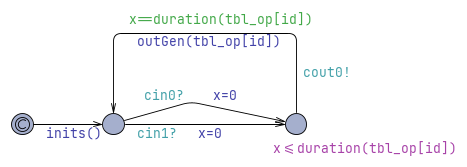
\includegraphics[width=0.6\textwidth]{obrazky-figures/model_gate2.png}
    \caption{Časový automat reprezentující model logického hradla}
    \label{fig:model_gate2}
\end{figure}

\subsection{Inicializace systému}
V závěru dochází k inicializace a propojení celého systému. Ve výpise \ref{lst:init} je vidět inicializace jednotlivých součástí. \texttt{synPri} představuje model synchronizace, \texttt{ediff} zase model kontroly rovnosti. \texttt{mul2A} je model přesné násobičky, \texttt{mul2Atb} představuje generátor náhodných vstupních hodnot. Na konci lze pozorovat inicializaci jednotlivých logických hradel \texttt{gate2}.

\begin{lstlisting}[language={C}, caption={Inicializace systému}, label={lst:init}]
synPri = syncPrimary();

mul2A = tmul2any(PIxy, POx, tbl_acc_any, DLY_MUL2);
mul2Atb = tmul2_tb_random(DLY_MUL2, COVERAGE_RATIO);

ediff = eval_diff(5);

//gates
g122=gate2(0, PIxy[14], PIxy[0], 122, change[14], change[0], change[122]);
g123=gate2(1, PIxy[15], PIxy[0], 123, change[15], change[0], change[123]);
g127=gate2(2, PIxy[10], PIxy[4], 127, change[10], change[4], change[127]);
g129=gate2(3, PIxy[13], PIxy[1], 129, change[13], change[1], change[129]);
g130=gate2(4, PIxy[14], PIxy[1], 130, change[14], change[1], change[130]);
g133=gate2(5, PIxy[15], PIxy[1], 133, change[15], change[1], change[133]);
g142=gate2(6, 122, 129, 142, change[122], change[129], change[142]);
//...
//...
//...
g433=gate2(214, 431, 430, 433, change[431], change[430], change[433]);
g434=gate2(215, 431, 430, POy[14], change[431], change[430], change[434]);
g435=gate2(216, 432, 433, POy[15], change[432], change[433], change[435]);
g436=gate2(217, 318, 210, POy[3], change[318], change[210], change[436]);
\end{lstlisting}

\section{Zvolená pravděpodobnostní rozdělení generování náhodných čísel} \label{rozdeleni_pst}

\section{Převod modelů z jazyku Verilog do modelů v nástroji UPPAAL} \label{parser}

\chapter{Výsledky experimentů}
\label{popis}
TODO

\chapter{Diskuze škálovatelnosti} 
\label{skalovatelnost}
TODO

\chapter{Závěr}
\label{zaver}
TODO

%===============================================================================

% Pro kompilaci po částech (viz projekt.tex) nutno odkomentovat
%\end{document}

